\chapter{Cubed-sphere grids}
\label{chp-cs-grids}
So far, we have described the dimension-splitting technique in Chapter \ref{chp-2d-fv} for solving the advection equation on the plane.
Our current goal is to apply these schemes to solve the advection equation on the sphere.
Consequently, we need to introduce a grid over the sphere.
In order to facilitate the extension of dimension-splitting techniques onto the sphere, we require a logical Cartesian coordinate system, at least locally.

We point out that dimension-splitting schemes could be formulated in unstruced grids (see for instance \citet{herzfeld:2023}).
A good reason to use a locally Cartesian grid is to avoid problems, such as the lack of convergence of the divergence operator among others,
that may arise in some grid cells within those grids \citep{peixoto:2013, peixoto:2016, weller:2012}.
Also, a logical Cartesian coordinate system eases the process of higher-order interpolation,
which can be more complicated on a spherical unstructured grid, requiring tangent plane approximations \citep{peixoto:2014,skamarock:2011}.

The scheme proposed by \citet{lin:1996} was originally implemented on latitude-longitude grids,
and the FV dynamical core was elucidated in \citet{lin:2004}.
The latitude-longitude grids exhibit convergence of meridians at the poles, 
necessitating the utilization of the Semi-Lagrangian formulation of PPM for larger CFL numbers,
as discussed in Section \ref{chp-adv1d-sec-flux}, 
to overcome the CFL restriction imposed by the poles.
However, this approach needs the processes in a parallel domain decomposition of the latitude-longitude grid to utilize more
data at the poles, resulting in non-parallel efficiency.
Therefore, \citet{putman:2007} proposed considering the cubed-sphere (CS, hereafter) instead.
The CS grid is more uniform, thus not exhibiting a strong CFL condition anywhere.
This eliminates the need for the Semi-Lagrangian formulation of PPM, which is better to parallel efficiency, and led to the development of the FV3 core.


The CS grid was originally proposed by \citet{sadourny:1972} and was 
reinvestigated by \citet{ronchi:1996} and \citet{rancic:1996}. 
As is usual for Planotic grids, we start with a Platonic solid, in this case, a cube, 
which is circumscribed in a sphere. We then project its faces onto the sphere.
The original CS, called the equidistant CS, was proposed by 
\citet{sadourny:1972} but resulted in a non-uniform grid. 
To address this issue, a solution was proposed by introducing angular coordinates, 
leading to a quasi-uniform grid known as the equiangular CS.
The cubed sphere consists of six panels, each one having a local Cartesian coordinate 
system. 
As we pointed out before, this makes it easier to extend methods from the plane to the sphere. 
In fact, \citet{putman:2007} extends the dimension splitting technique from 
\citet{lin:1996}, as presented in Chapter \ref{chp-2d-fv}, to the CS.

There are essentially two major challenges when working with the CS grid:
\begin{enumerate}
\item
The non-orthogonal grid system: This challenge is primarily related to the appearance of
metric terms in the equations. It adds computational cost and often requires conversions
between contravariant and covariant components of a velocity field.
\item
The discontinuity of the coordinate system at the cube edges: This is perhaps the most 
problematic challenge. Computing stencils along the cube edges becomes challenging due to 
the discontinuous nature of the coordinate system.
\end{enumerate}
One possible approach to compute stencils at the edges is to extend the local coordinate 
of each panel to its neighboring panels, adding ghost cells in the halo region. In the 
case of the equiangular CS, ghost cell values lie on the same geodesics 
containing the data from the neighboring panels. This allows for the use of one-dimensional
high-order Lagrange interpolation to compute the stencils at the edges. 
This approach has been extensively used in the literature \citep{croisille:2013, 
katta:2015, katta:2015b, chen:2021} and was initially introduced by \citet{ronchi:1996}.
This approach is referred to as \textbf{duo-grid}, as named by \citet{chen:2021}.
Alternatively, \citet{putman:2007} uses extrapolation for the PPM reconstruction values near the cube edges.
Another approach that avoids the need for interpolation or extrapolation near the edges is 
the conformal CS developed by \citet{rancic:1996}. While this grid leads to an 
orthogonal and continuous coordinate system near the edges, it generates grid singularities
near the cube corners, similar to the pole problem. 
An improved and more uniform conformal grid, called the Uniform Jacobian cubed sphere, was 
later proposed by \citet{rancic:2017}.
Each approach is likely to generate grid imprinting, and one of the goals of this work is 
to investigate the amount of grid imprinting produced by each method.

This Chapter aims to review and investigated the geometrical properties
of the CS. Besides that, we also aim to investigate the process
of interpolating/extrapolating near the cube edges.
We start with a basic review of the CS mappings in Section \ref{cs-mappings},
while Section \ref{cs-halodata} investigates how we can apply 1D Lagrange interpolation using the adjacent panels
data to obtain values of a scalar/vector field on ghost cells, as well different edge
treatments when computing stencils near to the cube edges.
Final thoughts are presented in Section \ref{cs-conc}.

\newpage
\section{Cubed-sphere mappings}
\label{cs-mappings}
\subsection{Mapping between the cube and sphere}
\label{equidistant-cs}
We start this section by introducing the mapping between the cube and the sphere, which will divide the sphere into 6 quadrilaterals, also called panels, and allow us to tessellate the sphere into smaller quadrilaterals for panels.
Given $R>0$, we denote the sphere of radius $R$ 
centered at the origin of  $\mathbb{R}^3$ as:
\begin{equation*}
	\mathbb{S}^2_R = \{ P = (X,Y,Z) \in \mathbb{R}^3: X^2 + Y^2 + Z^2 = R^2\}.
\end{equation*}
We consider a parameter %$a = \frac{R}{\sqrt{3}}$ representing the half-length of the cube,and
the family of maps
$\Psi_{p}: [-1,1] \times [-1,1] \to \mathbb{S}^2_R$, $p=1, \ldots, 6$,
where:
\begin{equation*}
	\Psi_{1}(x,y) = \frac{R}{\sqrt{1 + x^2 + y^2}}(1, x, y), 
\end{equation*}
\begin{equation*}
	\Psi_{2}(x,y) = \frac{R}{\sqrt{1 + x^2 + y^2}}(-x, 1, y), 
\end{equation*}
\begin{equation*}
	\Psi_{3}(x,y) = \frac{R}{\sqrt{1 + x^2 + y^2}}(-1, -x, y), 
\end{equation*}
\begin{equation*}
	\Psi_{4}(x,y) = \frac{R}{\sqrt{1 + x^2 + y^2}}(x, -1, y), 
\end{equation*}
\begin{equation*}
	\Psi_{5}(x,y) = \frac{R}{\sqrt{1 + x^2 + y^2}}(-y, x, 1), 
\end{equation*}
\begin{equation*}
	\Psi_{6}(x,y) = \frac{R}{\sqrt{1 + x^2 + y^2}}(y, x, -1).
\end{equation*}


The set of 6 maps $\{\Psi_{p}, p = 1, \ldots, 6\}$ allow us to cover the sphere (Figure \ref{chp-cs-equidistant}).
Here $p$ denotes a panel, and they are defined and orientated as Figure \ref{chp-cs-panels}
shows. Then, we can represent a point on the sphere using the cubed-sphere coordinates
$(x,y,p)$.
\begin{figure}[!htb]
	\centering
	\begin{subfigure}{0.42\textwidth}
		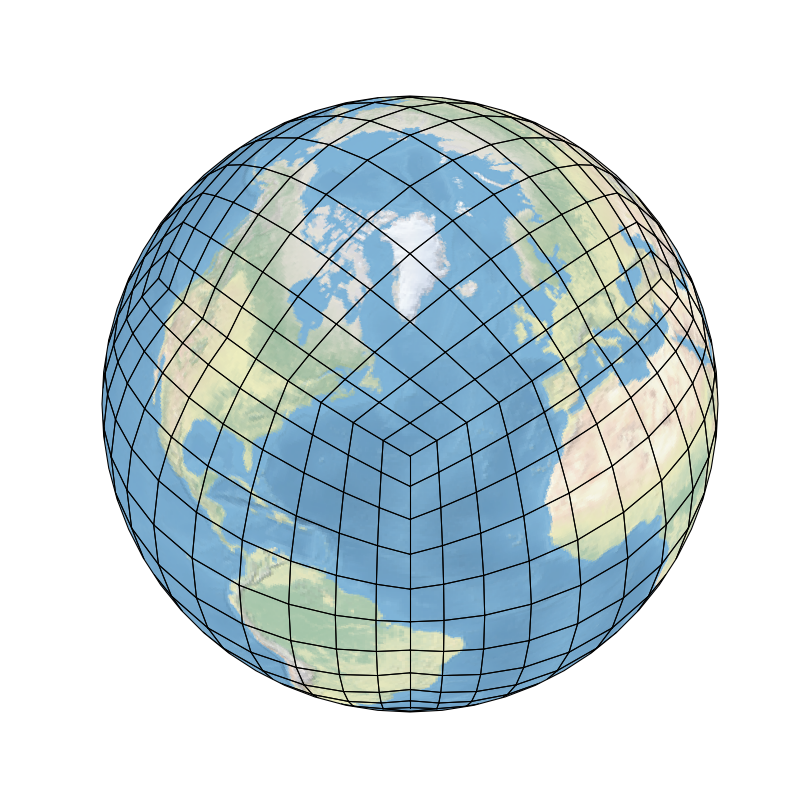
\includegraphics[width=0.8\linewidth]{gnomonic_equidistant_cs_10_sphere}
		\caption{Gridlines of the cube to the sphere mapping}
	\end{subfigure}
	\begin{subfigure}{0.42\textwidth}
		\centering
		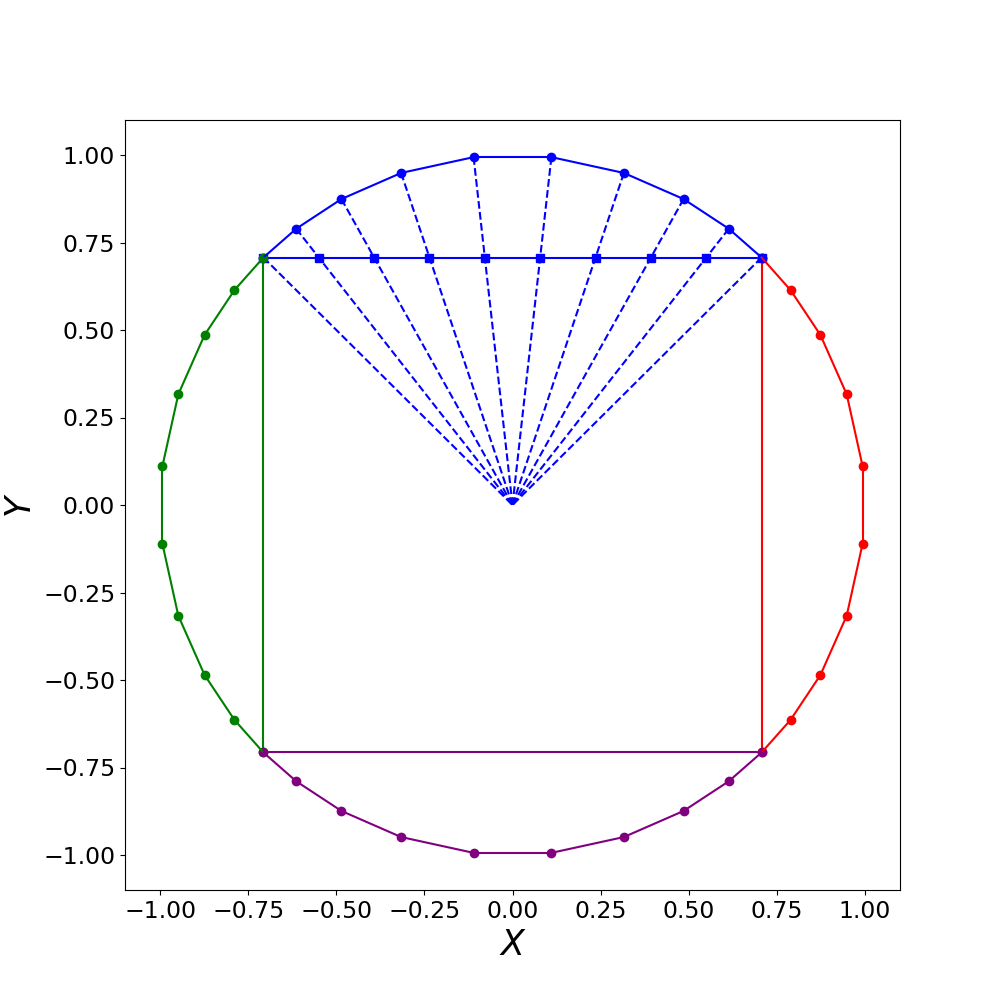
\includegraphics[width=0.8\linewidth]{g1}
		\caption{Cube and sphere mapping for $Z=0$.}
	\end{subfigure}
	\caption{(a) Illustration of the resulting cube-to-sphere mapping and (b) illustration of the cube-to-sphere projection.\label{chp-cs-equidistant}}
\end{figure}
\newpage
\begin{figure}[!htb]
	\centering
	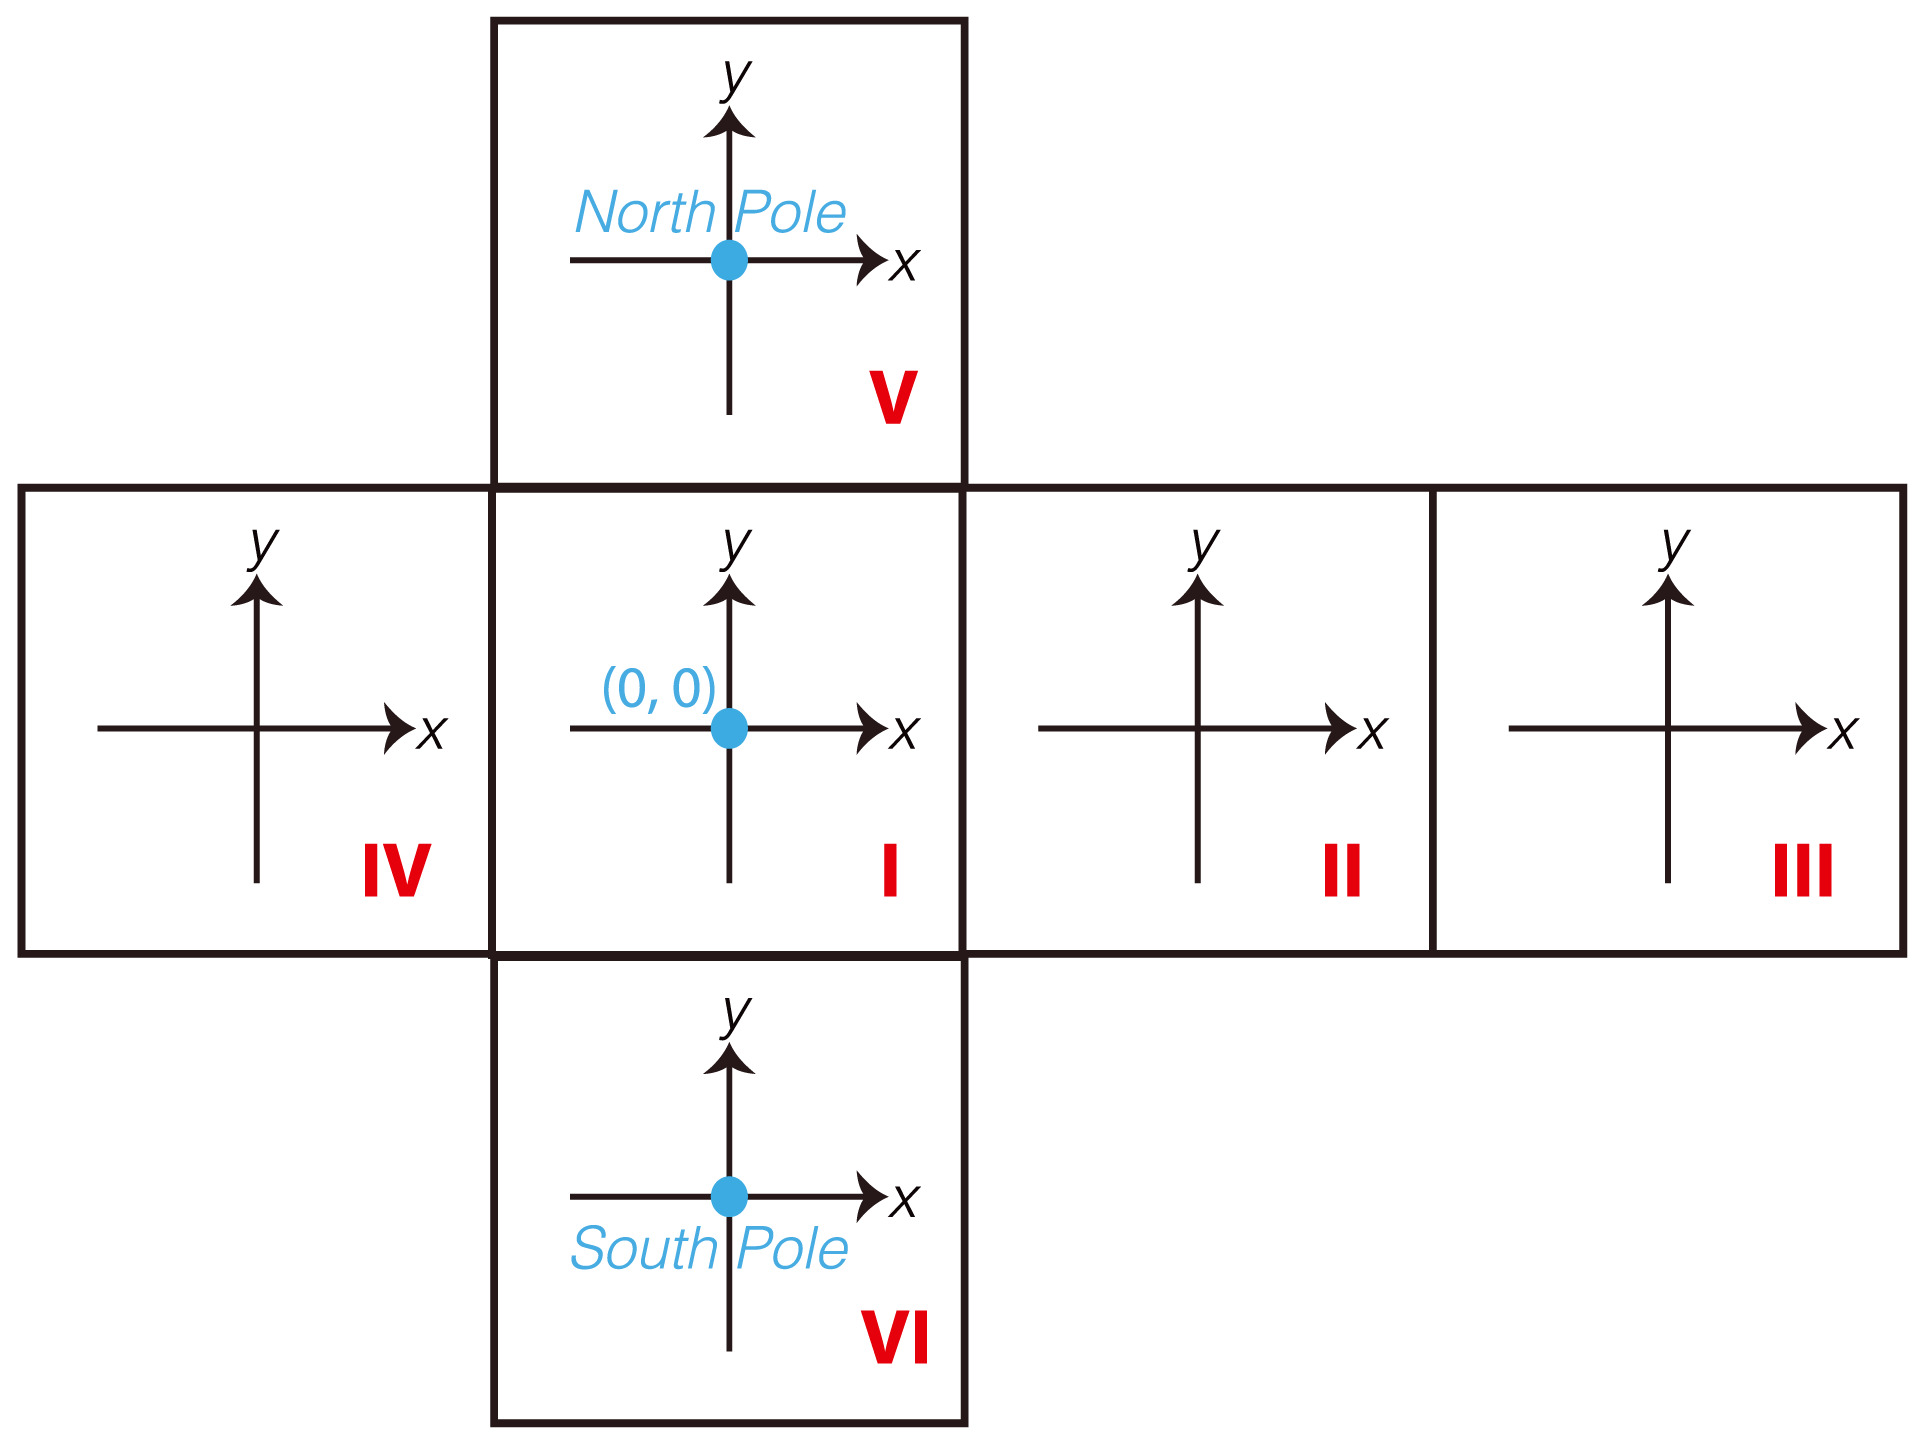
\includegraphics[width=0.4\linewidth]{chp4_panels}
	\caption{Cubed-sphere panels definition and orientation.
    Figure taken from \citet{jung:2019}.\label{chp-cs-panels}}
\end{figure}

The derivative of the maps $\Psi_p$ are given by:
\begin{equation*}
	d\Psi_{1}(x,y) = \frac{R}{{(1 + x^2 + y^2)}^{3/2}}
	\begin{bmatrix}
		-x & -y \\
	 	 1+y^2  & -xy \\
		 -xy  & 1+x^2
	\end{bmatrix},
\end{equation*}
\begin{equation*}
	d\Psi_{2}(x,y) = \frac{R}{{(1 + x^2 + y^2)}^{3/2}}
	\begin{bmatrix}
		-(1+y^2) & xy \\
		 -x &  -y \\
		 -xy &  1+x^2
	\end{bmatrix},
\end{equation*}
\begin{equation*}
	d\Psi_{3}(x,y) = \frac{R}{{(1 + x^2 + y^2)}^{3/2}}
	\begin{bmatrix}
		 x &  y \\
		-(1+y^2) & xy \\
		 -xy &  1+x^2
	\end{bmatrix},
\end{equation*}
\begin{equation*}
	d\Psi_{4}(x,y) = \frac{R}{{(1 + x^2 + y^2)}^{3/2}}	
	\begin{bmatrix}
		 1+y^2 &  -xy \\
		 x & y \\
		 -xy &  1+x^2
	\end{bmatrix},
\end{equation*}
\begin{equation*}
	d\Psi_{5}(x,y) = \frac{R}{{(1 + x^2 + y^2)}^{3/2}}	
	\begin{bmatrix}
		 xy  & -(1+x^2) \\
	 	 1+y^2  &  -xy \\
		-x & -y
	\end{bmatrix},
\end{equation*}
\begin{equation*}
	d\Psi_{6}(x,y) = \frac{R}{{(1 + x^2 + y^2)}^{3/2}}
	\begin{bmatrix}
		 -xy  &  1+x^2 \\
		 1+y^2  &  -xy \\
		 x &  y
	\end{bmatrix}.
\end{equation*}
With the aid of the derivative, we may define a basis of tangent vectors 
$\{\boldsymbol{\partial_x \Psi},  \boldsymbol{\partial_y \Psi}\}$ on each point on the sphere by:
\begin{equation*}
	\boldsymbol{\partial_x \Psi}(x,y,p) = d\Psi_{p}(x,y) \cdot
	\begin{bmatrix}
		 1 \\
		 0
	\end{bmatrix}, \quad
	\boldsymbol{\partial_y \Psi}(x,y,p) = d\Psi_{p}(x,y) \cdot
	\begin{bmatrix}
		 0 \\
		 1
	\end{bmatrix}.
\end{equation*}
Notice that the matrix
\begin{equation*}
	\label{chp-cs-eqdistant-Psitensor}
	G_{\Psi}(x,y) := 
	[d\Psi_{p}(x,y)]^Td\Psi_{p}(x,y)
	= \frac{R^2}{(1 + x^2 + y^2)^2}
	\begin{bmatrix}
		  1+ x^2 &  -xy \\
		 -xy & 1 + y^2
	\end{bmatrix},
\end{equation*}
does not depend on $p$.
This matrix is known as metric tensor.
It is easy to see that:
\begin{equation}
	\label{chp-cs-eqdistant-Psi-metric-tensor}
	G_{\Psi}(x,y) = 
	\begin{bmatrix}
		\langle  \boldsymbol{\partial_x \Psi}, \boldsymbol{\partial_x \Psi} \rangle & 
		\langle  \boldsymbol{\partial_x \Psi}, \boldsymbol{\partial_y \Psi} \rangle \\
		\langle  \boldsymbol{\partial_x \Psi}, \boldsymbol{\partial_y \Psi} \rangle  &
		\langle  \boldsymbol{\partial_y \Psi}, \boldsymbol{\partial_y \Psi} \rangle 
	\end{bmatrix},
\end{equation}
where $\langle \cdot, \cdot \rangle$ denotes 
the standard inner product of $\mathbb{R}^3$,
and that $G_{\Psi}(x,y)$ is positive-definite, 
$\forall (x,y) \in [-1,1]\times[-1,1]$.
The Jacobian of the metric tensor $G_{\Psi}(x,y)$, denoted by $\sqrt{g_{\Psi}}$ and called metric term, is then given by:
\begin{equation*}
        \sqrt{g_{\Psi}}(x,y) :=
	\sqrt{|\det{G_{\Psi}(x,y)}|} = \frac{R^2}{(1+x^2+y^2)^{3/2}}.
\end{equation*}
Now let us assume that we have a function $\beta:[-\alpha,\alpha] \to [-1,1]$, for some positive $\alpha>0$,
supposed to be bijective and $\mathcal{C}^1$ with inverse $\mathcal{C}^1$ as well.
Let us consider $\Phi_p: [-\alpha,\alpha]\times [-\alpha,\alpha] \to \mathbb{S}^2_R$,
given by $\Phi_p(x,y) := \Psi_p\big(\beta(x),\beta(y)\big)$.
It follows from the chain rule that:
\begin{equation*}
        d\Phi_p(x,y) = d\Psi_p\big(\beta(x),\beta(y)\big)\cdot\text{diag}\big(\beta'(x),\beta'(y)\big),
\end{equation*}
where $\text{diag}(\beta'(x),\beta'(y))$ is a diagonal $2\times 2$ matrix with diagonal entries given by $\beta'(x)$ and $\beta'(y)$.
We also have that tangent vector basis $\{\boldsymbol{\partial_x \Phi},  \boldsymbol{\partial_y \Phi}\}$ satisfying
\begin{align*}
	\boldsymbol{\partial_x \Phi}(x,y,p) = \beta'(x) \cdot \boldsymbol{\partial_x \Phi}\big(\beta(x),\beta(y),p\big),\\
	\boldsymbol{\partial_y \Phi}(x,y,p) = \beta'(y) \cdot \boldsymbol{\partial_y \Phi}\big(\beta(x),\beta(y),p\big).
\end{align*}
The metric tensor of $\Phi$ is defined as $G_{\Psi}$ in Equation \eqref{chp-cs-eqdistant-Psi-metric-tensor}:
\begin{equation*}
	\label{chp-cs-eqdistant-Phi-metric-tensor}
	G(x,y) = 
	\begin{bmatrix}
		\langle  \boldsymbol{\partial_x \Phi}, \boldsymbol{\partial_x \Phi} \rangle & 
		\langle  \boldsymbol{\partial_x \Phi}, \boldsymbol{\partial_y \Phi} \rangle \\
		\langle  \boldsymbol{\partial_x \Phi}, \boldsymbol{\partial_y \Phi} \rangle  &
		\langle  \boldsymbol{\partial_y \Phi}, \boldsymbol{\partial_y \Phi} \rangle 
	\end{bmatrix}.
\end{equation*}
Finally, the metric term $\sqrt{g}:= \sqrt{\det{G}}$ is expressed in terms of $\sqrt{g}_{\Psi}$ as
\begin{align*}
    \sqrt{g}(x,y) &= \beta'(x)\beta'(y)\sqrt{g}_{\Psi}\big(\beta(x),\beta(y)\big)\\
    &= \beta'(x)\beta'(y)\frac{R^2}{\big(1+\beta(x)^2+\beta(y)^2\big)^{3/2}}.
\end{align*}
Now that we have established between the cube and sphere, we may introduce the cubed-sphere grids proposed in the literature.

\subsection{Equidistant cubed-sphere}
\label{cs-equidistant}
The first cubed-sphere grid was proposed by \citet{sadourny:1972}. This grid is obtained by using
$\beta(x) = x$, $\alpha=1$ in the $\Phi_p$ mapping described in Section \ref{equidistant-cs}.
This grid partitions the cube face into equally spaced points
and projects them onto the sphere, as illustrated in Figure
\ref{chp-cs-equidistant}, hence the name equidistant.
We shall denote this grid by \textbf{g1} since the parameter
\textit{gridtype} in FV3 is set equal to 1 to use this grid.

\subsection{Equiangular cubed-sphere}
\label{cs-equiangular}
Another cubed-sphere mapping is the equiangular mapping, 
introduced by \citet{ronchi:1996}, which leads to a more uniform grid.
This grid is obtained by considering the mapping $\Phi_p$ described in Section \ref{equidistant-cs}
with $\beta(x) = \tan{x}$ and $\alpha=\frac{\pi}{4}$.
In this case, $\beta(x)$ represents the angular coordinates, and the cube-sphere is obtained by partitioning the angle between
grid points equally, as illustrated in Figure \ref{chp-cs-equiangular}, hence the name equiangular.
This grid is denoted by \textbf{g2}, for the same reason of the notation \textbf{g1}.
\begin{figure}[!htb]
	\centering
	\begin{subfigure}{0.42\textwidth}
		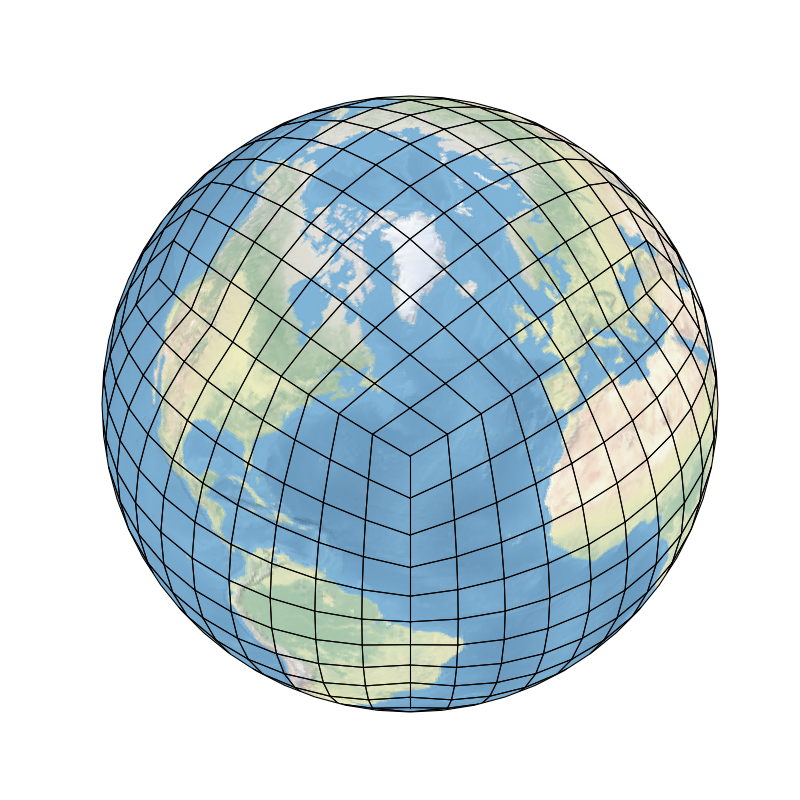
\includegraphics[width=0.8\linewidth]{gnomonic_equiangular_cs_10_sphere}
		\caption{Gridlines of the cube to the sphere equiangular mapping}
	\end{subfigure}
	\begin{subfigure}{0.42\textwidth}
		\centering
		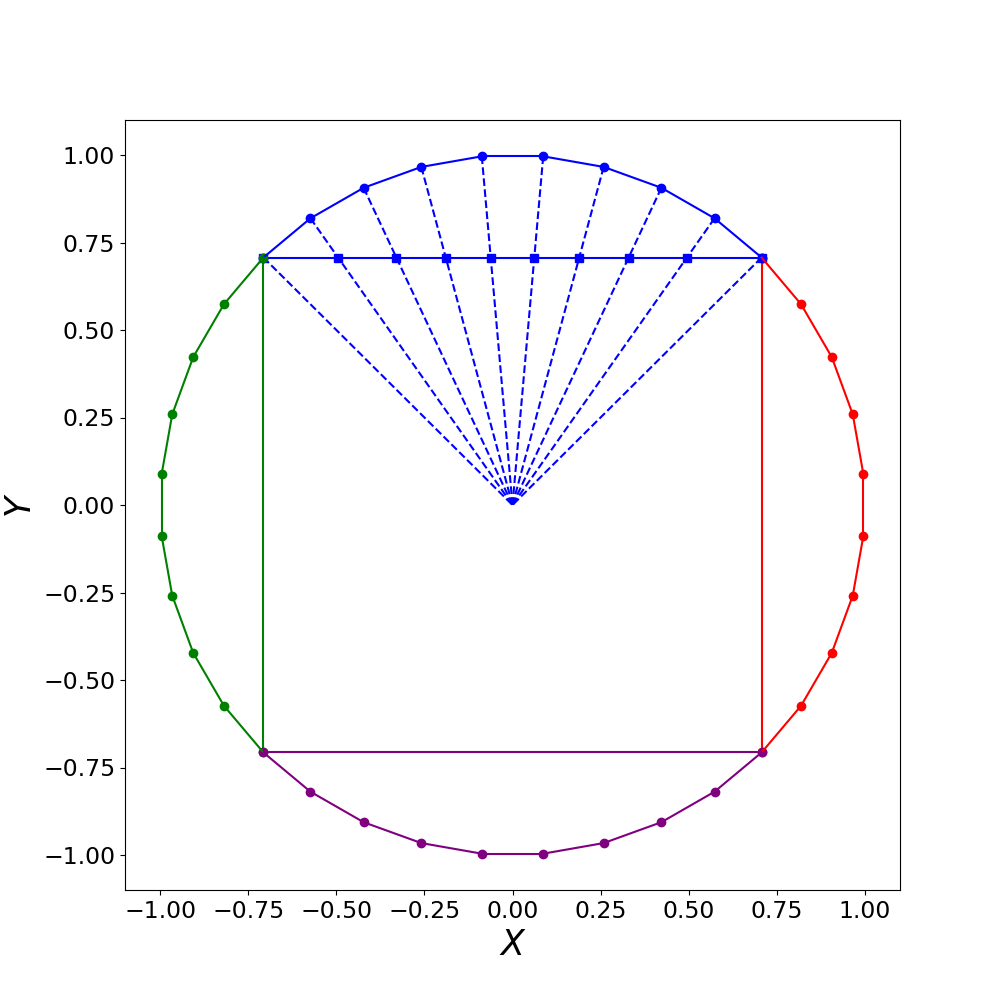
\includegraphics[width=0.8\linewidth]{g2}
		\caption{Cube and sphere equiangular mapping for $Z=0$.}
	\end{subfigure}
	\caption{(a) Illustration of the resulting cube-to-sphere mapping and (b) illustration of the cube-to-sphere projection using the equiangular mapping.\label{chp-cs-equiangular}}
\end{figure}

\subsection{Equiedge cubed-sphere}
\label{cs-equiedge}
An equiangular cubed-sphere modification 
\citet{chen:2021} by using $\beta(x) = \sqrt{2}\tan{x}$ and
$\alpha=\arcsin{\big(\frac{1}{\sqrt{3}}\big)}$.
Figure \ref{chp-cs-equiedge} illustrates the equiedge mapping.
\begin{figure}[!htb]
	\centering
	\begin{subfigure}{0.42\textwidth}
		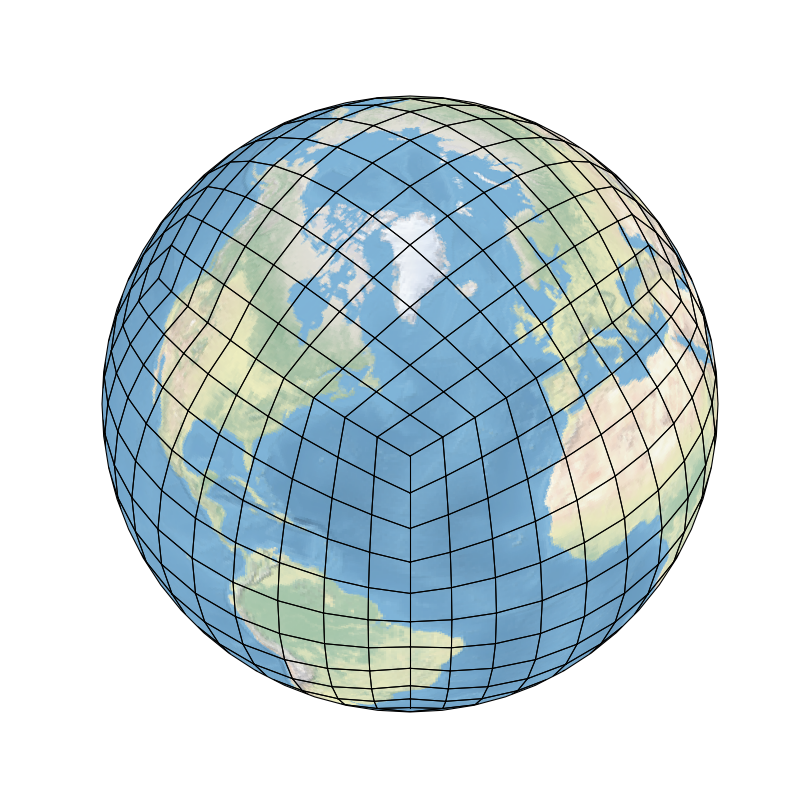
\includegraphics[width=0.8\linewidth]{gnomonic_equiedge_cs_10_sphere}
		\caption{Gridlines of the cube to the sphere equiedge mapping}
	\end{subfigure}
	\begin{subfigure}{0.42\textwidth}
		\centering
		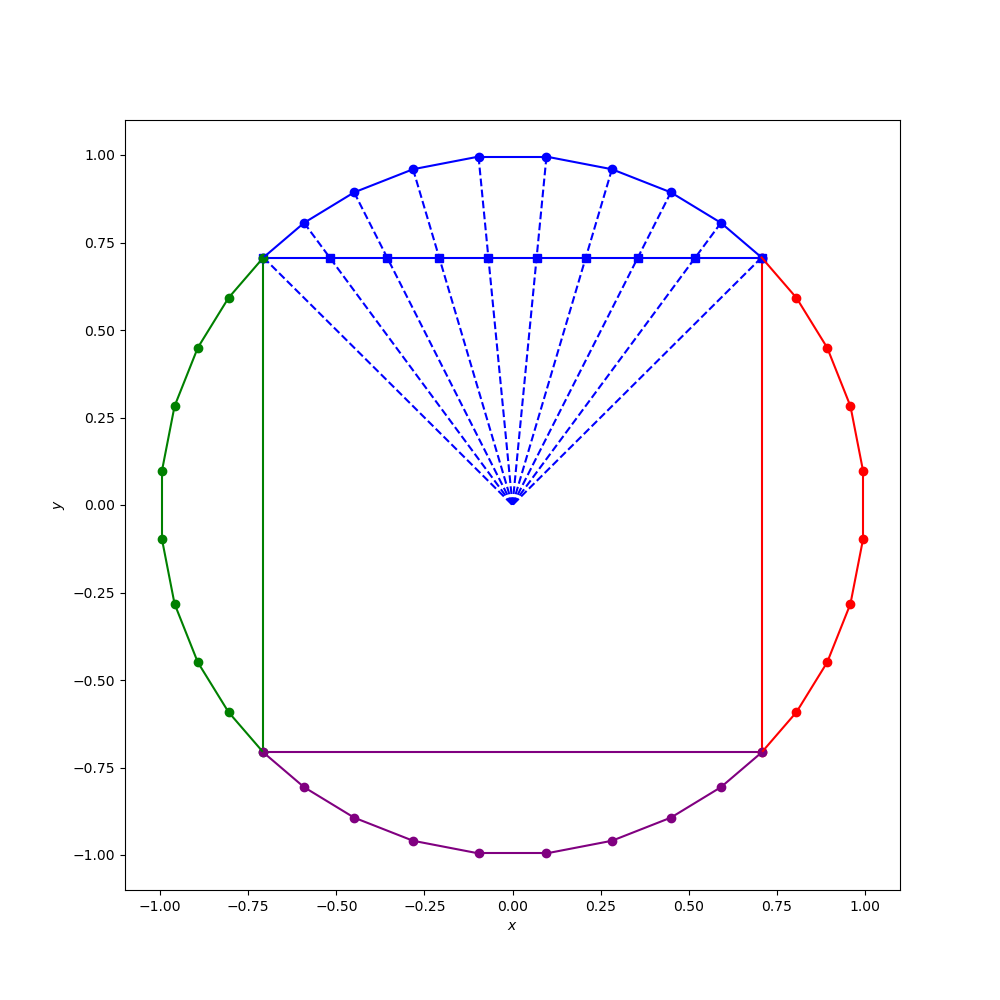
\includegraphics[width=0.8\linewidth]{g0}
		\caption{Cube and sphere equiedge mapping for $Z=0$.}
	\end{subfigure}
	\caption{(a) Illustration of the resulting cube-to-sphere mapping and (b) illustration of the cube-to-sphere projection using the equiedge mapping.\label{chp-cs-equiedge}}
\end{figure}
The idea behind lies in partitioning the edges of the spherical cube equally, and then generating the other cells,
hence the name equiedge.
This grid is denoted by \textbf{g0}, for the same reason of the notation \textbf{g1}.
Also, this grid leads to more uniform cells after applying the grid stretching option of FV3 \citep{harris:2016, chen:2021}.

\subsection{Geometric properties}
We will utilize the notation introduced in Section \ref{chp-adv2d-sec-not} throughout this Chapter.
We shall used the earth radius $R = 6.371 \times 10^6$ meters.
The parameter $\nu$ represents a non-negative integer indicating the number of ghost cell layers in each panel boundary, called halo size.

To generate the cubed-sphere, we consider a $(\Delta x, \Delta y)$-grid denoted by 
$\Omega_{\Delta x, \Delta y} = (\Omega_{ij})_{i,j=-\nu+1,\ldots,N+\nu}$, 
where $\Delta x = \Delta y$, and it covers the domain $\Omega$. 
A control volume of the cubed-sphere is denoted by $\Omega_{ijp}$, defined as follows:
\begin{equation*}
	\Omega_{ijp} = \Phi_p(\Omega_{ij})
	\quad -\nu+1 \leq i, j \leq N+\nu, \quad 1 \leq p \leq 6.
\end{equation*}
The cubed-sphere grid refers to the collection of control volumes 
$(\Omega_{ijp})_{i,j=-\nu+1,\ldots,N+\nu}^{p=1,\ldots,6}$. 
In Figures \ref{chp-cs-equidistant}, \ref{chp-cs-equiangular} and \ref{chp-cs-equiedge} examples of the cubed-sphere grids are depicted,
excluding the ghost cells.
These grids are generated using the equidistant, equiangular and equiedge mappings for $N=10$.

We will denote the area of $\Omega_{ijp}$ by $|\Omega_{ij}|$.
Notice that the area does not depend on the panel due to the grid symmetry.
We also define the diameter of a cell as $2\sqrt{\frac{|\Omega_{ij}|}{\pi}}$, which corresponds to the diameter of a circle with area $|\Omega_{ij}|$.

\begin{table}[htbp]
    \centering
    \caption{Mean diameter, minimum diameter, and maximum diameter for different values of $N$ considering the equiedge grid (g0).\label{g0-dx-table}}
    \begin{tabular}{cccccc}
        \toprule
        $N$ & Mean Length (km) & Min Length (km) & Max Length (km) & $\frac{\text{Max}}{\text{Min}}$ \\
        \midrule
        48 & 218.8099 & 175.2215 & 266.1879 & 1.5192 \\
        96 & 108.5933 & 86.6886 & 131.7271 & 1.5195 \\
        192 & 54.0963 & 43.1173 & 65.5228 & 1.5196 \\
        384 & 26.9983 & 21.5024 & 32.6764 & 1.5197 \\
        768 & 13.4868 & 10.7372 & 16.3170 & 1.5197 \\
        \bottomrule
    \end{tabular}
\end{table}

\begin{table}[htbp]
    \centering
    \caption{As Table \ref{g0-dx-table} but considering the equidistant grid (g1). \label{g1-dx-table}}
    \begin{tabular}{cccccc}
        \toprule
        $N$ & Mean Length (km) & Min Length (km) & Max Length (km) & $\frac{\text{Max}}{\text{Min}}$ \\
        \midrule
        48 & 215.2132 & 134.2046 & 305.7128 & 2.2780 \\
        96 & 107.0361 & 66.3960 & 151.3249 & 2.2791 \\
        192 & 53.3767 & 33.0242 & 75.2757 & 2.2794 \\
        384 & 26.6532 & 16.4690 & 37.5408 & 2.2795 \\
        768 & 13.3178 & 8.2238 & 18.7461 & 2.2795 \\
        \bottomrule
    \end{tabular}
\end{table}

\begin{table}[htbp]
    \centering
    \caption{As Table \ref{g0-dx-table} but considering the equiangular grid (g2). \label{g2-dx-table}}
    \begin{tabular}{cccccc}
        \toprule
        $N$ & Mean Length (km) & Min Length (km) & Max Length (km) & $\frac{\text{Max}}{\text{Min}}$ \\
        \midrule
        48 & 220.5051 & 202.0487 & 240.2358 & 1.1890 \\
        96 & 109.2509 & 99.9583 & 118.8660 & 1.1892 \\
        192 & 54.3786 & 49.7172 & 59.1234 & 1.1892 \\
        384 & 27.1281 & 24.7936 & 29.4847 & 1.1892 \\
        768 & 13.5488 & 12.3806 & 14.7231 & 1.1892 \\
        \bottomrule
    \end{tabular}
\end{table}

\begin{table}[htbp]
    \centering
    \caption{Mean area, minimum area, and maximum area for different values of $N$ considering the equiedge grid (g0).\label{g0-da-table}}
    \begin{tabular}{cccccc}
        \toprule
        $N$ & Mean Area (km$^2$) & Min Area (km$^2$) & Max Area (km$^2$) & $\frac{\text{Max}}{\text{Min}}$ \\
        \midrule
        48 & 38033.0342 & 24113.7560 & 55650.1616 & 2.3078 \\
        96 & 9364.8432 & 5902.1925 & 13628.2415 & 2.3090 \\
        192 & 2323.6050 & 1460.1378 & 3371.9038 & 2.3093 \\
        384 & 578.7202 & 363.1308 & 838.6059 & 2.3094 \\
        768 & 144.4087 & 90.5461 & 209.1068 & 2.3094 \\
        \bottomrule
    \end{tabular}
\end{table}

\begin{table}[htbp]
    \centering
    \caption{As Table \ref{g0-da-table} but considering the equidistant grid (g1). \label{g1-da-table}}
    \begin{tabular}{cccccc}
        \toprule
        $N$ & Mean Area (km$^2$) & Min Area (km$^2$) & Max Area (km$^2$) & $\frac{\text{Max}}{\text{Min}}$ \\
        \midrule
        48 & 37762.8967 & 14145.7139 & 73403.5750 & 5.1891 \\
        96 & 9331.7795 & 3462.3692 & 17985.0194 & 5.1944 \\
        192 & 2319.5149 & 856.5522 & 4450.4100 & 5.1957 \\
        384 & 578.2116 & 213.0213 & 1106.8685 & 5.1960 \\
        768 & 144.3452 & 53.1165 & 276.0003 & 5.1961 \\
        \bottomrule
    \end{tabular}
\end{table}

\begin{table}[htbp]
    \centering
    \caption{As Table \ref{g0-da-table} but considering the equidistant grid (g1). \label{g2-da-table}}
    \begin{tabular}{cccccc}
        \toprule
        $N$ & Mean Area (km$^2$) & Min Area (km$^2$) & Max Area (km$^2$) & $\frac{\text{Max}}{\text{Min}}$ \\
        \midrule
        48 & 38269.2622 & 32062.8284 & 45327.8673 & 1.4137 \\
        96 & 9393.6416 & 7847.4299 & 11096.9937 & 1.4141 \\
        192 & 2327.1605 & 1941.3433 & 2745.4160 & 1.4142 \\
        384 & 579.1619 & 482.8032 & 682.7832 & 1.4142 \\
        768 & 144.4637 & 120.3862 & 170.2515 & 1.4142 \\
        \bottomrule
    \end{tabular}
\end{table}

In tables \ref{g0-dx-table}, \ref{g1-dx-table}, and \ref{g2-dx-table},
we display the diameters of the grids g0, g1, and g2 for $N=48\times 2^k$, 
where $k = 0,\ldots, 4$. These values of $N$ are considered in this work.
Similarly, in tables \ref{g0-dx-table}, \ref{g1-dx-table}, and \ref{g2-dx-table}, we display the areas.

We can observe that in terms of areas and diameters of the cells, grid g1 is the least uniform,
while g2 is the most uniform grid.
Grid g0 is more uniform than g1, but the maximum/minimum ratio of the areas is almost 2.3.
Therefore, in this thesis, we shall constrain our attention to grid g2, since it is ideally more uniform.

\section{Tangent vectors on the sphere}
\label{cs-tgvectors}
The tangent space at $P \in \mathbb{S}^2_R$ is denoted by $T_P \mathbb{S}^2$.
It is easy to see that:
\begin{equation*}
	T_P\mathbb{S}^2_R = \{P_0 \in \mathbb{R}^3: \langle P,P_0\rangle = 0\}.
\end{equation*}
We are going to consider three ways to represent an element of $\mathbb{S}_R^2$:
using $(X,Y,Z)$ coordinates, or using $(\lambda, \phi)$
latitude-longitude coordinates, or, at last, using the cubed-sphere
coordinates $(x,y,p)$, where $(x,y)$ are the cube face coordinates and 
$p \in \{1,2,\cdots, 6\}$ stands for a cube panel.
We say that a vector field $\boldsymbol{u}: \mathbb{S}^2_R \to 
\mathbb{R}^3$ is tangent on  the sphere if
$\boldsymbol{u}(P) \in T_P\mathbb{S}^2_R$, $\forall P \in \mathbb{S}^2_R$.

\subsection{Conversions between latitude-longitude and contravariant coordinates}
\label{anexo-sph-ll}
We consider the latitude-longitude mapping 
$\Psi_{ll}: [0,2\pi] \times [-\frac{\pi}{2},\frac{\pi}{2}] \to \mathbb{S}^2_R$, given by:
\begin{align}
	\label{ll2sph}
	X(\lambda,\phi) &= R\cos \phi \cos \lambda,\\
	Y(\lambda,\phi) &= R\cos \phi \sin \lambda,\\
	Z(\lambda,\phi) &= R\sin \phi.
\end{align}
The derivative or Jacobian matrix of the mapping $\Psi_{ll}$ is given by:
\begin{equation}
	\label{dpsi}
	D\Psi_{ll} (\lambda,\phi) = 
	R \begin{bmatrix}
		-\cos \phi \sin \lambda &  -\sin \phi \cos \lambda \\
		\cos \phi \cos \lambda & \sin \phi \sin \lambda \\
		0  &  \cos \phi
	\end{bmatrix}.
\end{equation}
Using this matrix columns, we can define the tangent vectors:
\begin{equation}
	\boldsymbol{r}_{\lambda}(\lambda,\phi) = D\Psi_{ll}(\lambda,\phi)
	\begin{bmatrix}
		1 \\
		0
	\end{bmatrix}, \quad
	\boldsymbol{r}_{\phi}(\lambda,\phi) = D\Psi_{ll}(\lambda,\phi)
	\begin{bmatrix}
		0 \\
		1
	\end{bmatrix}.
\end{equation}
We normalize the vectors $\boldsymbol{r}_\lambda$ and $\boldsymbol{r}_\phi$
and we obtain unit tangent vectors on the sphere at $\Phi_{ll}(\lambda, \phi)$:
\begin{equation}
	\label{latlon_tg_vectors}
	\boldsymbol{e}_{\lambda}(\lambda,\phi) = 
	\begin{bmatrix}
		-\sin \lambda \\
		\cos \lambda \\
		0
	\end{bmatrix}, \quad
	\boldsymbol{e}_{\phi}(\lambda,\phi) =
	\begin{bmatrix}
		-\sin \phi \cos \lambda \\
		-\sin \phi \sin \lambda \\
		\cos \phi
	\end{bmatrix}.
\end{equation}
Let us consider a tangent vector field $\boldsymbol{u}: \mathbb{S}^2_R \to 
\mathbb{R}^3$ on the sphere, represented as
\begin{equation}
	\label{latlon-wind}
	\boldsymbol{u}(\lambda, \phi) = 
	u_{\lambda} (\lambda, \phi) \boldsymbol{e}_{\lambda} (\lambda, \phi) + 
	v_{\phi} (\lambda, \phi) \boldsymbol{e}_{\phi} (\lambda, \phi). 
\end{equation}
Or, we may also represent this vector field using the basis 
obtained by cubed-sphere coordinates:
\begin{equation}
	\label{contravariant-wind}
	\boldsymbol{u}(x, y, p) = 
	{u}(x, y, p) \boldsymbol{r}_{x}(x, y, p) + 
	{v}(x, y, p) \boldsymbol{r}_{y}(x, y, p).
\end{equation}
This representation is known as contravariant representation.
In order to relate the latitude-longitude representation
with the contravariant representation, we notice that:
\begin{align}
	\label{basis-convertion1}
	\boldsymbol{\partial_x \Phi_p}(x, y, p) &= 
	\langle \boldsymbol{r}_{x} , \boldsymbol{e}_{\lambda}\rangle
	\boldsymbol{e}_{\lambda} (\lambda, \phi)  
	+ \langle \boldsymbol{r}_{x} , \boldsymbol{e}_{\phi}\rangle
	\boldsymbol{e}_{\phi} (\lambda, \phi), \\
	\label{basis-convertion2}
	\boldsymbol{\partial_y \Phi_p}(x, y, p) &=  
	\langle \boldsymbol{r}_{y} , \boldsymbol{e}_{\lambda}\rangle
	\boldsymbol{e}_{\lambda} (\lambda, \phi) 
	+ \langle \boldsymbol{r}_{y} , \boldsymbol{e}_{\phi}\rangle
	\boldsymbol{e}_{\phi} (\lambda, \phi), 
\end{align}
which holds since the vectors $\boldsymbol{e}_{\lambda}(\lambda, \phi)$ and
$\boldsymbol{e}_{\phi}(\lambda, \phi)$ are orthogonal.
Replacing Equations \eqref{basis-convertion1} and \eqref{basis-convertion2}
in Equation \eqref{contravariant-wind}, we obtain the values $(u_\lambda, v_\phi)$
in terms of the contravariant components $({u},{v})$ 
as the following matrix equation:
\begin{equation}
	\label{ll-to-contravariant}
	\begin{bmatrix}
		u_\lambda (\lambda, \phi) \\
		v_\phi (\lambda, \phi) 
	\end{bmatrix}
	=
	\begin{bmatrix}
		\langle \boldsymbol{\partial_x \Phi_p}, \boldsymbol{e}_\lambda \rangle 
		& \langle \boldsymbol{\partial_y \Phi_p}, \boldsymbol{e}_\lambda \rangle \\
		\langle \boldsymbol{\partial_x \Phi_p}, \boldsymbol{e}_\phi \rangle 
		& \langle \boldsymbol{\partial_y \Phi_p}, \boldsymbol{e}_\phi \rangle \\
	\end{bmatrix}
	\begin{bmatrix}
		{u}(x,y,p) \\
		{v}(x,y,p)
	\end{bmatrix}.
\end{equation}
Conversely, we may express the contravariant components in terms of
latitude-longitude components by inverting Equation \eqref{ll-to-contravariant}:
\begin{equation}
	\label{contravariant-to-ll}
	\begin{bmatrix}
		{u}(x,y,p) \\
		{v}(x,y,p)
	\end{bmatrix}
	=
	\frac{1}{\langle \boldsymbol{\partial_x \Phi_p}, \boldsymbol{e}_\lambda\rangle
		\langle \boldsymbol{\partial_y \Phi_p}, \boldsymbol{e}_\phi \rangle
		-\langle \boldsymbol{\partial_y \Phi_p}, \boldsymbol{e}_\lambda \rangle
		\langle \boldsymbol{\partial_x \Phi_p}, \boldsymbol{e}_\phi \rangle}
	\begin{bmatrix}
		\langle \boldsymbol{\partial_y \Phi_p}, \boldsymbol{e}_\phi \rangle 
		&-\langle \boldsymbol{\partial_y \Phi_p}, \boldsymbol{e}_\lambda \rangle \\
		-\langle \boldsymbol{\partial_x \Phi_p}, \boldsymbol{e}_\phi \rangle 
		& \langle \boldsymbol{\partial_x \Phi_p}, \boldsymbol{e}_\lambda \rangle \\
	\end{bmatrix}
	\begin{bmatrix}
		u_\lambda (\lambda, \phi) \\
		v_\phi (\lambda, \phi) 
	\end{bmatrix}.
\end{equation}

\subsection{Covariant/contravariant conversion}
\label{anexo-cov-con}
Let us consider again a tangent vector field $\boldsymbol{u}: \mathbb{S}^2_R \to 
\mathbb{R}^3$ on the sphere. Its contravariant representation 
is given by Equation \eqref{contravariant-wind}.
The covariant components $(U,V)$ are given by:
\begin{align}
	\label{covariant-u}
	U(x,y,p) = \langle \boldsymbol{u}(x,y,p) , \boldsymbol{\partial_x \Phi_p}(x,y,p)  \rangle, \\
	\label{covariant-v}
	V(x,y,p) = \langle \boldsymbol{u}(x,y,p) , \boldsymbol{\partial_y \Phi_p}(x,y,p)  \rangle.
\end{align}
Replacing Equation \eqref{contravariant-wind} in 
Equations \eqref{covariant-u} and \eqref{covariant-v} we obtain
the relation covariant components in terms of the
contravariant terms:
\begin{equation}
	\label{contravariant-to-covariant}
	\begin{bmatrix}
		{U}(x,y,p) \\
		{V}(x,y,p)
	\end{bmatrix}
	=
	\begin{bmatrix}
		\langle \boldsymbol{\partial_x \Phi_p}, \boldsymbol{\partial_x \Phi_p} \rangle
		& \langle \boldsymbol{\partial_x \Phi_p}, \boldsymbol{\partial_y \Phi_p} \rangle \\
		\langle \boldsymbol{\partial_x \Phi_p}, \boldsymbol{\partial_y \Phi_p} \rangle 
		& \langle \boldsymbol{\partial_y \Phi_p}, \boldsymbol{\partial_y \Phi_p} \rangle \\
	\end{bmatrix}
	\begin{bmatrix}
		{u} (x,y,p) \\
		{v} (x,y,p) 
	\end{bmatrix}.
\end{equation}
We may express the contravariant components in terms of 
the covariant terms inverting Equation \eqref{contravariant-to-covariant}:
\begin{equation}
	\label{convariant-to-contravariant}
	\begin{bmatrix}
		{u}(x,y,p) \\
		{v}(x,y,p)
	\end{bmatrix}
	= \frac{1}{\langle \boldsymbol{\partial_x \Phi_p}, \boldsymbol{\partial_x \Phi_p} \rangle
		\langle \boldsymbol{\partial_y \Phi_p}, \boldsymbol{\partial_y \Phi_p} \rangle
		- \langle \boldsymbol{\partial_x \Phi_p}, \boldsymbol{\partial_y \Phi_p} \rangle^2}
	\begin{bmatrix}
		\langle \boldsymbol{\partial_y \Phi_p}, \boldsymbol{\partial_y \Phi_p} \rangle
		& -\langle \boldsymbol{\partial_x \Phi_p}, \boldsymbol{\partial_y \Phi_p} \rangle \\
		-\langle \boldsymbol{\partial_x \Phi_p}, \boldsymbol{\partial_y \Phi_p} \rangle 
		& \langle \boldsymbol{\partial_x \Phi_p}, \boldsymbol{\partial_x \Phi_p} \rangle \\
	\end{bmatrix}
	\begin{bmatrix}
		{U} (x,y,p) \\
		{V} (x,y,p) 
	\end{bmatrix}.
\end{equation}
Notice that combining Equations \eqref{contravariant-to-covariant}
and \eqref{convariant-to-contravariant} with Equations 
\eqref{ll-to-contravariant} and \eqref{contravariant-to-ll}
one may get relations between the latitude-longitude 
components and the covariant components.

\subsection{Notation}
\label{cs-notation}
We also utilize the notation $\mathcal{CS}_N=\mathbb{R}^{(N+\nu)\times(N+\nu)\times 6}$
to represent grid functions on the cubed-sphere at cell centers.
Let's assume we have a function $q:\mathbb{S}^2_R\times[0,T] \to \mathbb{R}$, 
and we have a $(\Delta x, \Delta y, \Delta t, \lambda)$-discretization of $\Omega \times [0,T]$.
We introduce $q^n \in \mathcal{CS}^N$, which represents the grid function $q$
evaluated at the discrete points. 
In other words, $q^n_{ijp} = q(x_i,y_j,p,t^n)$, where $i,j=-\nu +1, \ldots, N+\nu$, and $p=1, \ldots, 6$.
Furthermore, we use the notations $q^n_{i+\frac{1}{2},j,p} = q(x_{i+\frac{1}{2}},y_j, t^n)$ 
for $i=-\nu, \ldots, N+\nu$ and $j=-\nu +1, \ldots, N+\nu$ to represent $q$ at the midpoint of edges in
the $x$ direction.
Similarly, we use $q^n_{i,j+\frac{1}{2},p} = q(x_i,y_{j+\frac{1}{2}},t^n)$ for $i=-\nu +1, \ldots, N+\nu$ and $j=-\nu, \ldots, N+\nu$ to represent $q$ at the midpoint of edges in the $y$ direction.
When $q$ does not depend on the time variable $t$, we can omit the index $n$.
In Figure \ref{chp4-cs-grid-function}, we depict a grid function at centers, edge midpoints in the $x$ direction
and edge midpoints in the $y$ direction for the equiangular cubed-sphere considering
the halo size equal to three.

For a grid function $Q$ we also use the notations:
\begin{align*}
	Q_{\times,j,p} &:= (Q_{-\nu+1,j,p}, \ldots, Q_{N+\nu,j,p}) \in \mathbb{R}^{N}_{\nu},\\
	Q_{i,\times,p} &:= (Q_{i,-\nu+1,p}, \ldots, Q_{i,M+\nu,p}) \in \mathbb{R}^{N}_{\nu}.
\end{align*}
$|\Omega_{ijp}|$ is the control volume area given by:
\begin{equation}
	\label{chp4-area}
	|\Omega_{ijp}| = \int_{x_{i-\frac{1}{2}}}^{x_{i+\frac{1}{2}}} \int_{y_{j-\frac{1}{2}}}^{y_{j+\frac{1}{2}}}{\sigma(x,y)} \,dx \,dy.
\end{equation}
We define the average values of a function $q$ with the aid of the metric tensor
$\sigma(x,y)$ at time $t$: 
\begin{equation*}
	Q_{ijp}(t) = \frac{1}{|\Omega_{ijp}|}\int_{x_{i-\frac{1}{2}}}^{x_{i+\frac{1}{2}}}
	\int_{y_{j-\frac{1}{2}}}^{y_{j+\frac{1}{2}}}  q(x,y,p,t) {\sigma(x,y)}\,dx \,dy,
\end{equation*}
In this context, we define $Q(t) \in \mathcal{CS}_N$ given by 
$Q(t) = (Q_{ijp}(t))_{i,j = -\nu +1, \ldots, N+\nu}^{p=1,\ldots,6}$.
Similar to Proposition \ref{prop-bound-centroid-2d}, we may approximate the average value using the centroid value, that is
\begin{equation*}
	Q_{ijp}^n - q_{ijp}^n = O(\Delta x ^2), 
\end{equation*}
In this work, we shall always approximate the average values since our schemes are expected to be at most second-order,
this approximation does not deteriorate the convergence order.

\section{Edges treatment}
\label{cs-halodata}

\section{Concluding remarks}
\label{cs-conc}
